\documentclass[11pt]{amsart}
\usepackage{geometry}                % See geometry.pdf to learn the layout options. There are lots.
\geometry{letterpaper}                   % ... or a4paper or a5paper or ... 
%\geometry{landscape}                % Activate for for rotated page geometry
%\usepackage[parfill]{parskip}    % Activate to begin paragraphs with an empty line rather than an indent
\usepackage{graphicx}
\usepackage{amssymb}
\usepackage{epstopdf}
\DeclareGraphicsRule{.tif}{png}{.png}{`convert #1 `dirname #1`/`basename #1 .tif`.png}
\usepackage{amsfonts,amsmath,amsthm,amsbsy,latexsym,amssymb,graphicx,booktabs,multicol,color,fullpage}
\usepackage{mathabx,dashrule}
\usepackage{manfnt}
\usepackage{pgf,tikz}
\usepackage{pgfplots}
\usepackage{graphicx}
\usepackage{wrapfig}
\usepackage{multicol}
\usepackage{arydshln}



\title{A Numerically Stable Fourier Continuation Approximation for the Solution of Partial Differential Equations}
\author{Melanie Vining}
%\date{}                                           % Activate to display a given date or no date

\begin{document}
\maketitle
\section{Introduction} \\
\subsection{Motivation} \\
Our goal is to study a numerically accurate and stable scheme for solving partial differential equations on complex domains.  Several finite difference and finite element methods are available but have low-order accuracy.  We focus on the Fourier-Continuation Alternating-Direction (FC-AD)  method described by Bruno and Lyon in (citation needed!). This method gives a high-order unconditionally stable solver for partial differential equations on any smooth domain.  One of the interesting details in the FC-AD method is that the modification to the solution that yields unconditional stability is neither inherent to the problem nor an obvious choice and was in fact developed by numerical experiment.  We aim to find an unconditional stability condition that is more natural either to the problem itself or to the mechanics of the implementation (analyzing the singular values of the matrix, for example).  
\subsubsection{FC-AD}
The Fourier-Continuation Alternating-Direction algorithm is a method that applies the concept of Alternating Direction Implicit (ADI) methods to using a Fourier Continuation (FC) method in the spatial domain.  ADI methods reduce the numerical solution to PDEs into implicit first order boundary value problems in space.  In traditional ADI methods, these  BVPs are solved using finite-difference methods and yield low-accuracy results on the boundaries.  

\subsubsection{FC Gram}
The FC Gram method matches points on a grid and applies a precomputed extension that results in a periodic function.  This resulting function can then be transformed via Fast Fourier Transform (FFT) in order to take derivatives.
\subsubsection{Fourier Continuation}

\section{Current Work}
We study the Boundary Value Problem (BVP) $(I-\alpha \frac{\partial^2}{\partial x^2})u=f$ with boundary values $u(a)=u_0$ and $u(b)=u_1$.  Our goal is to find the ``best" Fourier Continuation Approximation that we can use to approximate $f$ such that when we invert the operator to solve for $\tilde{u}$ (numerically) the result is stable, i.e. $\frac{\|\tilde{u}\|_{\ell^2}}{\|\tilde{f}\|_{\ell^2}} \leq 1$.  \\
The trouble we run into is that the Fourier Continuation Approximation can take any form in the continuation domain, as long as the result has the correct period (see Figure). 
\begin{figure}
\begin{center}
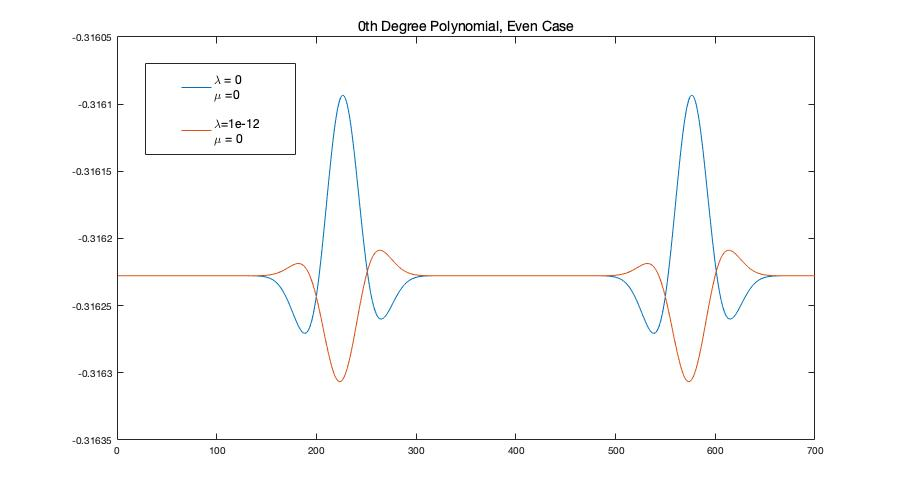
\includegraphics[scale = .4]{VariousConts0degEven.jpg}
\caption{Two different Fourier Continuations for a degree 0 polynomial. Both give approximately 16 digits of accuracy.}
\label{fig:Fig1}
\end{center}
\end{figure}
This means that it is possible for a procedure to ``choose" a Fourier Continuation Approximation for which energy builds in the continuation region, and then will spread back into the original domain under the inverted operator.  This can cause an unstable result.  In Figure \ref{fig:Fig1} we see that for no trade in accuracy, the blue line gives us an unstable result, while the red line gives us a stable result. \\

\subsection{What We've Done} 
We originally planned to explore the Singular Value Decomposition (SVD) of the system and try to exploit the zero singular values, but that proved to be ineffective in changing the shape of the continuation.  \\
We determined that by adding extra constraints to the system we're solving, we will be able to have more control over the system in question. Some fruitful results have come from focusing on a known solution to the BVP: The Green's Function. For simplicity, we assume that $a=-1$ and $b=b$ and that we have zero Boundary Conditions (BCs). 
\subsubsection{Green's Functions}
We calculate the Green's Function via the methods described in Bender and Orszag: Let 
\begin{equation}
G(x,a)=\begin{cases}
A_1(a)h_1(x)+B_1(a)h_2(x) & x<a \\
A_2(a)h_1(x)+B_2(a)h_2(x) & x \geq a
\end{cases}
\end{equation}
where $h_1(x)$ and $h_2(x)$ are the homogeneous solutions to  $(I-\alpha \frac{\partial^2}{\partial x^2})u=f$:
\begin{eqnarray}
h_1(x) &=& e^{\frac{(x-b)}{\sqrt{\alpha}}} \\
h_2(x) &=& e^{\frac{(-x-1)}{\sqrt{\alpha}}},
\end{eqnarray}
where $h_1$ and $h_2$ have been normalized to $1$ on the boundary.  $A_1$,$A_2$,$B_1$, and $B_2$ are computed to enforce continuity of the Green's Function, at most a small jump discontinuity of the Green's Function, and zero boundary conditions. 
To calculate the Green's Function solution to the BVP we use
\begin{equation}
u_G=\int_{-1}^b G(x,a)f(a)da.
\end{equation}
We then force the Fourier Continuation to match the function itself, and then force the inverted differential operator to match the Green's Function solution.  Since the Green's Function solution enforces zero BCs, we actually set up the equation to allow for fluctuation using the homogeneous solutions as-is, i.e. that  $(I-\alpha \frac{\partial^2}{\partial x^2})^{-1}f + a_1 h_1 + a_2 h_2 = u_G$. \\
Discretized on our grid, we use a Discrete Fourier Transform (DFT) Matrix, called $A$ to represent the Fourier Continuation operation, and $D$ to represent the differential operator.  The resulting system of equations is: 


\begin{equation}
\left[
\begin{array}{c:c}
A &  \mathbf{0} \\[6pt] \hdashline
(DA)^{\dagger} & h_1|_{\text{grid}} h_2|_{\text{grid}} \\[6pt]
\end{array} \right] 
\left[ 
\begin{array}{c}
f_c \\
a_1\\
a_2
\end{array}
\right]
= 
\left[ 
\begin{array}{c}
f|_{\text{grid}}\\
u_G|_{\text{grid}}
\end{array}
\right]
\end{equation}





\subsubsection{Enforcing Stability Via Homogeneous Solutions}
We found that the system above didn't always give us the stability we desired. To remedy this, we force a weight towards the Green's Function Solution by allowing the coefficients of that equation to be larger.  We achieve this by exploiting the fact that the SVD of the system will minimize the coefficients and adding the equation $\lambda a_1 h_1 + \lambda a_2 h_2 = 0$ to the system.  By taking $\lambda$ small, $a_1$ and $a_2$ will be larger.  By appropriately choosing $\lambda$ we are able to control the continuation and achieve stability. 

\subsection{Results} 
\section{Future Work} 
\subsection{Computational Work} 
We are going to use this to put as a time step of the heat equation and solve that PDE.  Our goal is to show that we have a stable approximation that can be used. 
\subsection{Analytical Work} \\
The result that yields the same Fourier coefficients for any given Gram polynomial independent of choice of $\alpha$ is unexpected.  Our goal is to develop an analytic proof that justifies this result in general. 



\end{document}  